\documentclass[12pt]{article}

\usepackage{amssymb}
\usepackage{physics}
%\usepackage{hyperref} % for hyperlinks in references
\usepackage[notref,notcite,color]{showkeyskay}\definecolor{labelkey}{rgb}{1,0,0.5}

\usepackage{graphicx}
\usepackage{caption} % for \caption*
\usepackage{mdframed} % for framed text and formulas
\usepackage[dvipsnames]{xcolor}

\numberwithin{equation}{section}

\newcommand{\be}{\begin{equation}}
\newcommand{\ee}{\end{equation}}
\newcommand{\e}{\mbox{e}}
\newcommand {\mm}[1]{\quad\mbox{#1}\quad}
\newcommand {\MM}[1]{\qquad\mbox{#1}\qquad}

\textwidth 170mm
\textheight 230mm
\voffset = -20mm

\title{Overview: a cell fluid model with Curie-Weiss interaction}

\author{R.V.~Romanik
	\\ \small Institute for Condensed Matter Physics, NAS of Ukraine
	\\ \small 1~Svientsitskii Street, 79011, Lviv, Ukraine
	\\ \small romanik@icmp.lviv.ua}
%\author{R.V.~Romanik \\ Institute for Condensed Matter Physics, NAS of Ukraine}

\begin{document}
	
	\maketitle
	
	%\begin{multicols}{2}
	
	\abstract{Review of the cell fluid model with Curie-Weiss interaction.
		\\	
		\textbf{Keywords:} Cell fluid model, Curie-Weiss interaction.
	}
	\section{Introduction}
	The cell model was introduced and described in~\cite{KKD18,KKD20}. This model possesses an exact solution in the case of Curie-Weiss interaction. The exact asymptotic expression for the grand partition function was obtained in~\cite{KKD20}.
	The goal of this manuscript is to summarize the notation, properly account for quantity dimensions corresponding to physical problems.
	
	\section{\label{sec:model} Model}
	Let us briefly introduce the model, the notation, and then summarize the known results for the model.
	
	The main results are obtained within the formalism of the grand canonical ensemble. An open system of point particles is considered in volume $V$. The total volume $V$ is divided into $N_v$ congruent cubic cells $\Delta_l$ of volume $v=c^3$ each, such that the volume $V$ is the union of all $\Delta_l$
	\begin{equation*}
		V = \bigcup_{l=1}^{N_v}\Delta_l,
	\end{equation*}
	and for each pair of $\Delta_l$ and $\Delta_m$
	\begin{equation*}
		\Delta_l \cap \Delta_m = \emptyset, \text{ if } l \neq m.
	\end{equation*}
	
	\textbf{Interaction.} The interaction energy between particles in configuration $\gamma = \{x_1, ..., x_N\}$, where $x_i$ is the space coordinate of the $i$-th particle and $N$ is the number of points (particles) in the configuration $\gamma$, is defined as follows
	\begin{equation*}
		W_{N_v}(\gamma) = \frac{1}{2} \sum_{x,y \in \gamma} \Phi_{N_v} (x,y)
	\end{equation*}
	where $\Phi_{N_v}$ is given by the Curie-Weiss interaction
	\begin{equation}
		\label{def:curie-weiss-pot}
		\Phi_{N_v}(x, y) = -\frac{J_1}{N_v} + J_2\sum_{l=1}^{N_v} I_{\Delta_l}(x) I_{\Delta_l}(y),
	\end{equation}
	and $I_{\Delta_l}(x)$ is the indicator of $\Delta_l$
	\begin{equation}
		\label{def:I}
		I_{\Delta_l} (x) = \left\{
		\begin{array}{ll}
			1, \quad x \in \Delta_l,
			\\
			0, \quad x \notin \Delta_l.
		\end{array}
		\right.
	\end{equation}
	The first term in $\Phi_{N_v}$ describes the pairwise attraction between all particles and is characterized by $J_1 > 0$. The second term in $\Phi_{N_v}$ describes the repulsion between two particles contained within the same cell $\Delta_l$ and is characterized by $J_2 > 0.$ For convenience, in $W_{N_v}$ above the self-interaction term $\Phi_{N_v}(x,x)$ is included, which does not affect the physics of the model. Two cases are possible, either two particles belong to the same cell or to different ones. Explicitly, one has
	\begin{equation}
		\Phi_{N_v}(x, y) = \left\{
		\begin{array}{ll}
			-\frac{J_1}{N_v} + J_2, & \text{when particles are in the same cell,}
			\\
			-\frac{J_1}{N_v}, & \text{otherwise.}
		\end{array}
		\right.
	\end{equation}
	In~\cite{KKD20}, the notation $\abs{\gamma}$ was used to denote the number of points (particles) in configuration $\gamma$, thus $\abs{\gamma} \equiv N$.
	
	\begin{mdframed}[linecolor=black,linewidth=1pt,leftline=true]
	If the notation from~\cite{HansenMcDonald13} is followed, the previous formulas can be rewritten as follows. The space coordinate of the $i$-th particle is denoted by $\vb{r}_i$, and thus the configuration of $N$ particles is defined by $\gamma = \{\vb{r}^N\}$, where $\vb{r}^N \equiv \vb{r}_1, ..., \vb{r}_N$. The interaction energy is expressed as (cf.~\cite[eq.~(2.5.16)]{HansenMcDonald13})
	\begin{eqnarray*}
		W_{N_v}(\vb{r}^N) & = & \frac{1}{2} \sum_{\vb{r}_i,\vb{r}_j \in \gamma} \Phi_{N_v} (\vb{r}_i,\vb{r}_j).
		\\
		& = & \frac12 {\sum_{i=1}^N \sum_{j=1}^N} \Phi_{N_v} (\vb{r}_i,\vb{r}_j),
	\end{eqnarray*}
	with
	\begin{equation*}
		\Phi_{N_v}(\vb{r}_i, \vb{r}_j) = -\frac{J_1}{N_v} + J_2\sum_{l=1}^{N_v} I_{\Delta_l}(\vb{r}_i) I_{\Delta_l}(\vb{r}_j),
	\end{equation*}
	and
	\begin{equation*}
		I_{\Delta_l} (\vb{r}) = \left\{
		\begin{array}{ll}
			1, \quad \vb{r} \in \Delta_l,
			\\
			0, \quad \vb{r} \notin \Delta_l.
		\end{array}
		\right.
	\end{equation*}
	Unlike~\cite[eq.~(2.5.16)]{HansenMcDonald13}, we do not exclude term with $i = j$ in the expression for $W_{N_v}$ due to the self-interaction.
	\end{mdframed}
	
	\textbf{Stability.} For stability of interaction the following condition must hold
	\begin{equation*}
		J_2 > J_1
	\end{equation*}
	to satisfy such inequality~\cite{KKD20,Ruelle70}
	\begin{equation}
		\int_{V} \Phi_{N_v}(x,y) {\rm d}y > 0, \quad \text{for all } x \in V.
	\end{equation}
	Note that there is one contribution to this integral from a cell containing the coordinate $x$, and $(N_v - 1)$ contributions from other cells:
	\begin{eqnarray*}
		\int_{V} \Phi_{N_v}(x,y) {\rm d}y & = & \left(-\frac{J_1}{N_v} + J_2\right)v - (N_v - 1) \frac{J_1}{N_v}v
		\\
		& = & (J_2 - J_1)v > 0.
	\end{eqnarray*}
	The ratio of the two energy constants is denoted by
	$$a = J_2/J_1,$$
	and thus $a > 1.$
	
	\textbf{The grand partition function} (GPF) is expressed as follows~\cite[eqs.~(2.4.6) and~(2.3.13)]{HansenMcDonald13}
	\begin{equation*}
		\Xi = \sum_{N=0}^{\infty}\frac{z^N}{N!} \int_{V} \dotsc \int_{V} \exp(-\beta W_{N_v}(\gamma)) {\rm d} x_1 \dotsc {\rm d} x_N
	\end{equation*}
	where $z$ is the activity
	\begin{equation*}
		z = \frac{\exp(\beta \mu)}{\Lambda^3},
	\end{equation*}
	$\beta = k_{\rm B} T$ the inverse temperature, $k_{\rm B}$ the Boltzmann constant, $T$ the temperature, $\mu$ the chemical potential, $\Lambda = (2\pi\beta\hbar^2/m)^{1/2}$ the de Broglie thermal wavelength, $\hbar$ the Planck constant, $m$ the mass of a particle. In GPF the integration goes over all configurations with $N$ particles and then the summation goes over all positive integer values of $N$.
	
	\begin{mdframed}[linecolor=black,linewidth=1pt,leftline=true]
		Alternatively, in notation from~\cite{HansenMcDonald13}, the GPF is expressed as [cf. eqs.~(2.4.6) and~(2.3.13)]
		\begin{equation}\label{ZGR}
			\Xi=\sum_{N=0}^{\infty}\frac{z^N}{N!}Z_N,
		\end{equation}
		where $Z_N$ is the configuration integral:
		\begin{equation}
			Z_N = \int\exp(-\beta W_{N_v}(\vb{r}^N)){\rm d}\vb{r}^N
		\end{equation}
		with ${\rm d} \vb{r}^N \equiv {\rm d}{\vb r_1} \dotsc {\rm d}{\vb r_N}$.
	\end{mdframed}
	
	\textbf{Reduced quantities.} Natural units for energy and length in the model are $J_1$ and $c$, respectively. It is standard practice to express thermodynamic results in terms of dimensionless quantities normalized by these natural units. The advantage of using such quantities is that their numerical values are typically of the order of unity, which simplifies analysis. Thus, we introduce the following reduced quantities:
	%the reduced temperature $T^* = k_{\rm B} T / J_1$, the reduced inverse temperature $p = \beta J_1$, reduced chemical potential $\mu^* = \mu / J_1$, and the reduced pressure $P^* = Pv/J_1$.
	\begin{eqnarray*}
		T^* := \frac{k_{\rm B} T}{J_1} & \quad & \text{ -- the reduced temperature;} 
		\\
		p := \beta J_1 = \frac{1}{T^*} & \quad & \text{ -- the reduced inverse temperature;}
		\\
		\mu^* := \frac{\mu}{J_1} & \quad & \text{ -- the reduced chemical potential;}
		\\ 
		P^* := \frac{Pv}{J_1} & & \text{ -- the reduced pressure.}
		\\
		S^* := \frac{S}{N_v k_{\rm B}} & & \text{ -- the reduced entropy.}
	\end{eqnarray*}
	For any dimensional quantity $Q$, it is convenient to denote its reduced counterpart by $Q^*$. To maintain consistency with other thermodynamic quantities, it may be beneficial to use $\beta^*$ instead of $p$ for the reduced inverse temperature (cf.~\cite{RDGMR13}).
	
	\subsection{Partition function transformation}
	Note the following summation:
	\begin{equation}
		\sum_{x,y \in \gamma} 1 = N^2 = \abs{\gamma}^2.
	\end{equation}
	The GPF is then explicitly written as
	\begin{equation}
		\label{eq:gpf1}
		\Xi = \sum_{N=0}^{\infty} \frac{\Lambda^{-3N}}{N!}\int \exp[\beta\mu N + \frac{p}{2N_{v}} N^2 - \frac{ap}{2} \sum_{x,y \in \gamma} \sum_{l=1}^{N_v} \mathbb{I}_{\Delta_l}(x)\mathbb{I}_{\Delta_l}(y)] {\rm d} x_1 \dotsc {\rm d} x_N.
	\end{equation}
	
	\begin{mdframed}[linecolor=black,linewidth=1pt,leftline=true]
	Alternatively
		\begin{equation}
			\label{eq:gpf1_alt}
			\Xi = \sum_{N=0}^{\infty} \frac{\Lambda^{-3N}}{N!}
			\int
			\exp[\beta\mu N + \frac{\beta^*}{2N_{v}} N^2 - \frac{a\beta^*}{2} \sum_{\vb{r}_i,\vb{r}_j \in \gamma} \sum_{l=1}^{N_v} \mathbb{I}_{\Delta_l}(\vb{r}_i)\mathbb{I}_{\Delta_l}(\vb{r}_j)] {\rm d} \vb{r}^N.
		\end{equation}
	\end{mdframed}
	Equations~\eqref{eq:gpf1} and~\eqref{eq:gpf1_alt} can be compared with~\cite[(2.5)]{KKD20}.
	
	For a given $l = 1, \cdots , N_v$ and a configuration $\gamma$, we set $\gamma_l = \gamma \cap \Delta_l,$ that is, $\gamma_l$ is the part of the configuration contained in $\Delta_l$. Then, $N_l$ or $\abs{\gamma_l}$ stands for the number of points (particles) of $\gamma$ contained in $\Delta_l$.
	
	\textbf{Some useful formulas}. Note the following summation results:
	\begin{equation}
		\label{eq:1}
		N_l \equiv \abs{\gamma_l} = \sum_{x \in \gamma_l} 1 = \sum_{x \in \gamma} \mathbb{I}_{\Delta_l}(x) = \sum_{j=1}^{N} \mathbb{I}_{\Delta_{l}}(x_j),
	\end{equation}
	\textbf{\textcolor{Red}{Question:}} Can $x \in \gamma_l$ and $x \in \Delta_l$ be used interchangeably?
	\begin{equation}
		\label{eq:2}
		\sum_{l=1}^{N_v} N_l = N, \quad \sum_{l=1}^{N_v} \abs{\gamma_l} = \abs{\gamma},
	\end{equation}
	\begin{equation}
		\label{eq:3}
		\left(\sum_{l=1}^{N_v} N_l \right)^2 = N^2, \quad \left(\sum_{l=1}^{N_v} \abs{\gamma_l} \right)^2 = \abs{\gamma}^2.
	\end{equation}
	\begin{equation}
		\label{eq:4}
		\sum_{x \in \gamma} \rightarrow \sum_{l=1}^{N_v} \sum_{x \in \Delta_l};
	\end{equation}
	\begin{equation}
		\label{eq:5}
		\sum_{x,y \in \gamma} \rightarrow \sum_{l,l'=1}^{N_v} \sum_{x \in \Delta_l} \sum_{y \in \Delta_{l'}}.
	\end{equation}
	\begin{equation}
		\label{eq:6}
		\sum_{x \in \Delta_l}\sum_{y \in \Delta_l'} 1 = N_l N_{l'} = \abs{\gamma_l} \abs{\gamma_{l'}}.
	\end{equation}
	\begin{equation}
		\label{eq:sumII}
		\sum_{x,y \in \gamma}\sum_{l=1}^{N_v} \mathbb{I}_{\Delta_l}(x) \mathbb{I}_{\Delta_{l}}(y) = \sum_{l=1}^{N_v} N_l^2 \equiv \sum_{l=1}^{N_v} \abs{\gamma_l}^2.
	\end{equation}
	Combining these formulas, we get
	\begin{eqnarray}
		\sum_{x,y \in \gamma} \Phi_{N_v}(x,y) & = & \sum_{l,l'=1}^{N_v} \sum_{x \in \Delta_l} \sum_{y \in \Delta_{l'}} \Phi_{N_v}(x,y)
		\nonumber\\
		& = & - \frac{J_1}{N_v} \left(\sum_{l=1}^{N_v} N_l\right)^2 + J_2\sum_{l=1}^{N_v}N_l^2
		\\
		& = & - \frac{J_1}{N_v} \left(\sum_{l=1}^{N_v} \abs{\gamma_l}\right)^2 + J_2\sum_{l=1}^{N_v}\abs{\gamma_l}^2
	\end{eqnarray}
	
	\textbf{GPF transformation}. To rewrite the integrand in~\eqref{eq:gpf1} in a more convenient form we set (cf.~\cite[eq.~(2.7)]{KKD20})
	\begin{equation}
		F_{N_v}(\varrho, p, \mu) = \exp[\frac{p}{2N_v}\left(\sum_{l=1}^{N_v} \varrho_l\right)^2 + \beta\mu\sum_{l=1}^{N_v} \varrho_l - \frac{a p}{2} \sum_{l=1}^{N_v} \varrho_l^2],
	\end{equation}
	where $\varrho \in \mathbb{N}_0^N$ is a vector with nonnegative integer components $\varrho_l$, $l=1, 2, \ldots , N_v$, i.e. $\varrho = (\varrho_1, \varrho_2, \ldots, \varrho_{N_{v}})$.
	
	For $\varrho$, we substitute the vector $\nu(\gamma) \in \mathbb{N}_0^N$ with components $N_l$ (or $\abs{\gamma_l}$), which have the meaning of the number of points in a cell $\Delta_{l}$ in cofiguration $\gamma$, i.e. $\nu(\gamma)=(N_1, N_2, \ldots, N_{N_v})$ or $\nu(\gamma) = (\abs{\gamma_1}, \abs{\gamma_2}, \ldots, \abs{\gamma_{N_v}})$, and obtain the following expression for the GPF in~\eqref{eq:gpf1}:
	\begin{equation}
		\Xi = \sum_{N=0}^{\infty} \frac{\Lambda^{-3N}}{N!}\int_{V^N} F_{N_v}(\nu(\gamma),p,\mu) {\rm d} x_1 \dotsc {\rm d} x_N,
	\end{equation}
	which can be compared with~\cite[eq.~(2.8)]{KKD20}.
	
	The next step is to intorduce the Kronecker $\delta$-symbol for $n, m \in \mathbb{N}_0$ as
	\begin{equation}
		\delta_{nm} = \int_0^1 \exp[2\pi {\rm i} t (n-m)] {\rm d}t
	\end{equation}
	and rewrite $F_{N_v}$ as
	\begin{equation}
		F_{N_v}(\nu(\gamma),p,\mu) = \sum_{\varrho \in \mathbb{N}_0^{N_v}} F_{N_v}(\varrho, p, \mu) 
		\int\limits_{[0,1]^{N_v}} \exp[2\pi{\rm i} \sum_{l=1}^{N_v} (\varrho_l - N_l)t_l ] {\rm d} t_1 \ldots {\rm d} t_{N_v},
	\end{equation}
	to arrive at (cf.~\cite[(2.9)]{KKD20})
	\begin{eqnarray}
		\label{eq:XiR}
		\Xi & = &  \sum_{\varrho \in \mathbb{N}_0^{N_v}} F_{N_v}(\varrho, p, \mu) 
		\sum_{N=0}^{\infty} \frac{\Lambda^{-3N}}{N!} 
		\nonumber\\
		&& \times \int\limits_{V^N} \int\limits_{[0,1]^{N_v}} 
		\exp[2\pi{\rm i} \sum_{l=1}^{N_v} (\varrho_l - N_l)t_l ] {\rm d} t_1 \ldots {\rm d} t_{N_v} {\rm d}x_1 \ldots {\rm d}x_N 
		\nonumber\\
		& = & \sum_{\varrho \in \mathbb{N}_0^{N_v}} F_{N_v}(\varrho, p, \mu)
		\int\limits_{[0,1]^{N_v}} \exp(2\pi{\rm i} \sum_{l=1}^{N_v} \varrho_l t_l) R_{N_v}(t_1, \ldots, t_{N_v}) {\rm d} t_1 \ldots {\rm d} t_{N_v}.
	\end{eqnarray}
	The summation over $\varrho$ is understood as
	\begin{equation}
		\sum_{\varrho \in \mathbb{N}_0^{N_v}} = \sum_{\varrho_1=0}^{\infty} \ldots \sum_{\varrho_{N_v}=0}^{\infty}.
	\end{equation}
	The quantity $R_N$ is expressed as follows (cf.~\cite[(2.10)]{KKD20})
	\begin{eqnarray}
		\label{def:RN}
		R_{N_v}(t_1, \ldots, t_{N_v}) & = & \sum_{N=0}^{\infty} \frac{\Lambda^{-3N}}{N!} \int\limits_{V^N} \exp(-2\pi{\rm i} \sum_{l=1}^{N_v} N_l t_l) {\rm d}x_1 \ldots {\rm d}x_N
		\nonumber\\
		&=& \sum_{N=0}^{\infty} \frac{\Lambda^{-3N}}{N!} \int\limits_{V^N} \exp(-2\pi{\rm i} \sum_{l=1}^{N_v} \sum_{j=1}^{N} \mathbb{I}_{\Delta_{l}}(x_j) t_l) {\rm d}x_1 \ldots {\rm d}x_N,
	\end{eqnarray}
	We used~\eqref{eq:1} to get the last line in the above equation.
	
	Note that the expression under the integral in the last line of~\eqref{def:RN} is factorized in $j$:
	\begin{eqnarray}
		R_{N_v}(t_1, \ldots, t_{N_v}) & = & \sum_{N=0}^{\infty}\frac{1}{N!} 
		\left\{\frac{1}{\Lambda^{3}} \int\limits_V \exp[-2\pi{\rm i}\sum_{l=1}^{N_v} \mathbb{I}_{\Delta_{l}}(x) t_l] {\rm d}x \right\}^N.
	\end{eqnarray}
	Applying the following transformation for the integral over $V$
	\begin{equation}
		\int\limits_V \ldots {\rm d}x = \sum_{l=1}^{N_v}\int\limits_{\Delta_l} \ldots {\rm d}x,
	\end{equation}
	and taking into account the definition of $\mathbb{I}_{\Delta_l}$~\eqref{def:I}, one gets for $R_{N_v}$
	\begin{eqnarray}
		\label{eq:RNL}
		R_{N_v}(t_1, \ldots, t_{N_v}) & = & \sum_{N=0}^{\infty}\frac{1}{N!} \left[ \frac{1}{\Lambda^3} \sum_{l=1}^{N_v} \int\limits_{\Delta_l} \exp(-2\pi{\rm i}t_l) {\rm d}x \right]^N
		\nonumber\\
		&=& \exp[\frac{v}{\Lambda^3} \sum_{l=1}^{N_v} \exp(-2\pi{\rm i} t_l)].
	\end{eqnarray}
	Here we used an obvious result $\int_{\Delta_l} {\rm d}x = v$. It is natural to introduce
	\begin{equation}
		v^* = \frac{v}{\Lambda^3},
	\end{equation}
	and write down the final expression for $R_{N_v}$
	\begin{equation}
		\label{eq:RNv}
		R_{N_v}(t_1, \ldots, t_{N_v}) = \exp[v^* \sum_{l=1}^{N_v} \exp(-2\pi{\rm i} t_l)].
	\end{equation}
	Compare this expression with the corresponding one in~\cite[p.~4]{KKD20} 
	
	Let us substitute~\eqref{eq:RNv} into~\eqref{eq:XiR}
	\begin{equation}
		\label{eq:XiIntt}
		\Xi(p,\mu) = \sum_{\varrho \in \mathbb{N}_0^{N_v}} F_{N_v}(\varrho, p, \mu) \prod\limits_{l=1}^{N_v} \int\limits_{0}^{1} \exp[2\pi{\rm i}\varrho_l t_l + v^* \exp(-2\pi{\rm i} t_l)] {\rm d} t_l.
	\end{equation}
	Here, the integral gives the following result:
	\begin{equation}
		\label{integral1}
		\int\limits_{0}^{1} \exp[2\pi{\rm i}\varrho_l t_l + v^* \exp(-2\pi{\rm i} t_l)] {\rm d} t_l = \frac{{(v^*)}^{\varrho_l}}{\varrho_l !}.
	\end{equation}
	\textbf{\textcolor{Red}{NOTE:}} This integral has not been explicitly written down in any of the papers~\cite{KKD18, KKD20, KD22}, and I do not know how it is calculated. However, I have determined that this result was implicitly substituted into~\cite[(2.11)]{KKD20}. I have verified this using Maple, and it yields the result given in~\eqref{integral1}.
	
	The GPF takes on the form (cf.~\cite[2.11]{KKD20}):
	\begin{eqnarray}
		\label{eq:XiPi}
		\Xi(p,\mu) & = & \sum_{\varrho \in \mathbb{N}_0^{N_v}} F_{N_v}(\varrho, p, \mu) \prod\limits_{l=1}^{N_v} \frac{(v^*)^{\varrho_l}}{\varrho_l !}
		\nonumber\\
		& = & \sum_{\varrho \in \mathbb{N}_0^{N_v}} \exp[\frac{p}{2 N_v} \left(\sum_{l=1}^{N_v} \varrho_l\right)^2] \prod\limits_{l=1}^{N_v} \pi(\varrho_l, \mu),
	\end{eqnarray}
	where
	\begin{equation}
		\label{def:pirho}
		\pi(\varrho_l, \mu) = \frac{(v^*)^{\varrho_l}}{\varrho_l !} \exp(\beta\mu\varrho_l - \frac{ap}{2}\varrho_l^2), \quad \varrho_l \in \mathbb{N}_0.
	\end{equation}
	\begin{mdframed}[linecolor=black,linewidth=1pt,leftline=true]
		In a generic form
		\begin{equation}
			\label{def:pin}
			\pi(n, \mu) = \frac{(v^*)^n}{n!} \exp(\beta\mu n - \frac{ap}{2}n^2), \quad n \in \mathbb{N}_0.
		\end{equation}
	\end{mdframed}
	
	\textbf{The Poisson distribution} results from~\eqref{def:pin} at $p=0$, i.e. in the high-temperature limit. To see this, rewrite expression for $\pi(n,\mu)|_{p=0}$ as
	\begin{equation}
		\pi(n,\mu)|_{p=0} = {\rm e}^{v^* {\rm e}^{\beta\mu}} 
		\frac{\left(v^* {\rm e}^{\beta\mu}\right)^n}{n!} {\rm e}^{-v^* {\rm e}^{\beta\mu}} 
		= {\rm e}^{v^* {\rm e}^{\beta\mu}} f(n; \lambda)
	\end{equation}
	where the (non-normalized) Poisson distribution $f(n; \lambda)$ is given by
	\begin{equation}
		f(n; \lambda) = \frac{\lambda^n {\rm e}^{-\lambda}}{n!}, \quad \lambda = v^* {\rm e}^{\beta\mu}.
	\end{equation}
	
	\textbf{Further transformation}. Applying the Gaussian integral
	\begin{equation}
		\int\limits_{-\infty}^{\infty} {\rm e}^{-\alpha y^2 + \beta y} {\rm d}y = \sqrt{\frac{\pi}{\alpha}} {\rm e}^{\frac{\beta^2}{4\alpha}},
	\end{equation}
	explicitly to Eq.~\eqref{eq:XiPi}
	\begin{equation}
		\label{eq:gaussInt}
		\exp[\frac{p}{2N_v}\left(\sum_{l=1}^{N_v} \varrho_l\right)^2] = \sqrt{\frac{N_v}{2\pi p}}
		\int\limits_{-\infty}^{\infty} \exp(-N_v \frac{y^2}{2p} + y\sum_{l=1}^{N_v} \varrho_l) {\rm d}y
	\end{equation}
	we transform~\eqref{eq:XiPi} into the following expression
	\begin{equation}
		\label{eq:XiInty}
		\Xi (p, \mu) = \sqrt{\frac{N_v}{2\pi p}} \int\limits_{-\infty}^{\infty} \exp[N_v E(y, p, \mu)] {\rm d} y,
	\end{equation}
	where 
	\begin{equation}
		\label{def:E}
		E(y,p,\mu) = -\frac{y^2}{2p} + \ln K(y,p,\mu),
	\end{equation}
	with
	\begin{equation}
		\label{def:K}
		K(y,p,\mu) = \sum_{n=0}^{\infty} \frac{(v^*)^n}{n!} \exp[(y+\beta\mu)n - \frac{ap}{2}n^2].
	\end{equation}
	Explicit derivation of expressions for $E(y,p,\mu)$ and $K(y,p,\mu)$ is given in Appendix~\ref{sec:app1}.
	
	\textbf{Some reasoning on numerical value of $v^*$.} During particular calculations, a numerical value for $v^*$ must be chosen. Which value to select may depend on physical reasoning. The dependence of results on $v^*$ may also be investigated.
	
	Since $v^* = c^3/\Lambda^3$, we may focus on a choice for $c$. One approach to choosing $c$ is in such a way that a classical consideration is justified. For example, it can be taken as the mean nearest-neighbour separation, see~\cite[Sec.~1.1]{HansenMcDonald13}. From the data given in~\cite[Table~1.1]{HansenMcDonald13}, the ratio $c/\Lambda$ may vary between $3.8$ and $59$ (we ignored data for $H_2$, as quantum effects are important for this substance). This defines possible values for $v^*$ as ranging between $57$ and $2 \cdot 10^5$.
	
	\textbf{Constraint on $E(y,p,\mu)$}. From inequality
	\begin{equation}
		\left(\frac{y+\beta\mu}{ap} - n\right)^2 \geq 0
	\end{equation}
	it follows
	\begin{equation}
		(y+\beta\mu)n - \frac{ap}{2}n^2 \leq \frac{(y+\beta\mu)^2}{2ap}.
	\end{equation}
	The last inequality, in turn, leads to corresponding inequalities for $K(y,p,\mu)$
	\begin{eqnarray}
		K(y,p,\mu) & \leq & \sum_{n=0}^{\infty}\frac{(v^*)^n}{n!} \exp[\frac{(y+\beta\mu)^2}{2ap}]
	\end{eqnarray}
	or
	\begin{equation}
		K(y,p,\mu) \leq \exp[\frac{(y+\beta\mu)^2}{2ap}] \exp(v^*),
	\end{equation}
	and for $E(y,p,\mu)$
	\begin{equation}
		\label{ineq:E0}
		E(y,p,\mu) \leq -\frac{a-1}{2ap}y^2 + \frac{\beta\mu}{2ap}(2y+\beta\mu) + v^*.
	\end{equation}
	Since $a>1$, \eqref{ineq:E0} implies the following limits for fixed $p$ and $\mu$
	\begin{equation}
		\lim_{y \to -\infty} E(y,p,\mu) = -\infty, \quad \lim\limits_{y \to +\infty} E(y,p,\mu) = -\infty.
	\end{equation}
	Typical behavior of $E(y,p,\mu)$ as a function of $y$ in the single-phase domain is illustrated in Fig.~\ref{fig:E0_vs_y}
	\begin{figure}[htbp]
		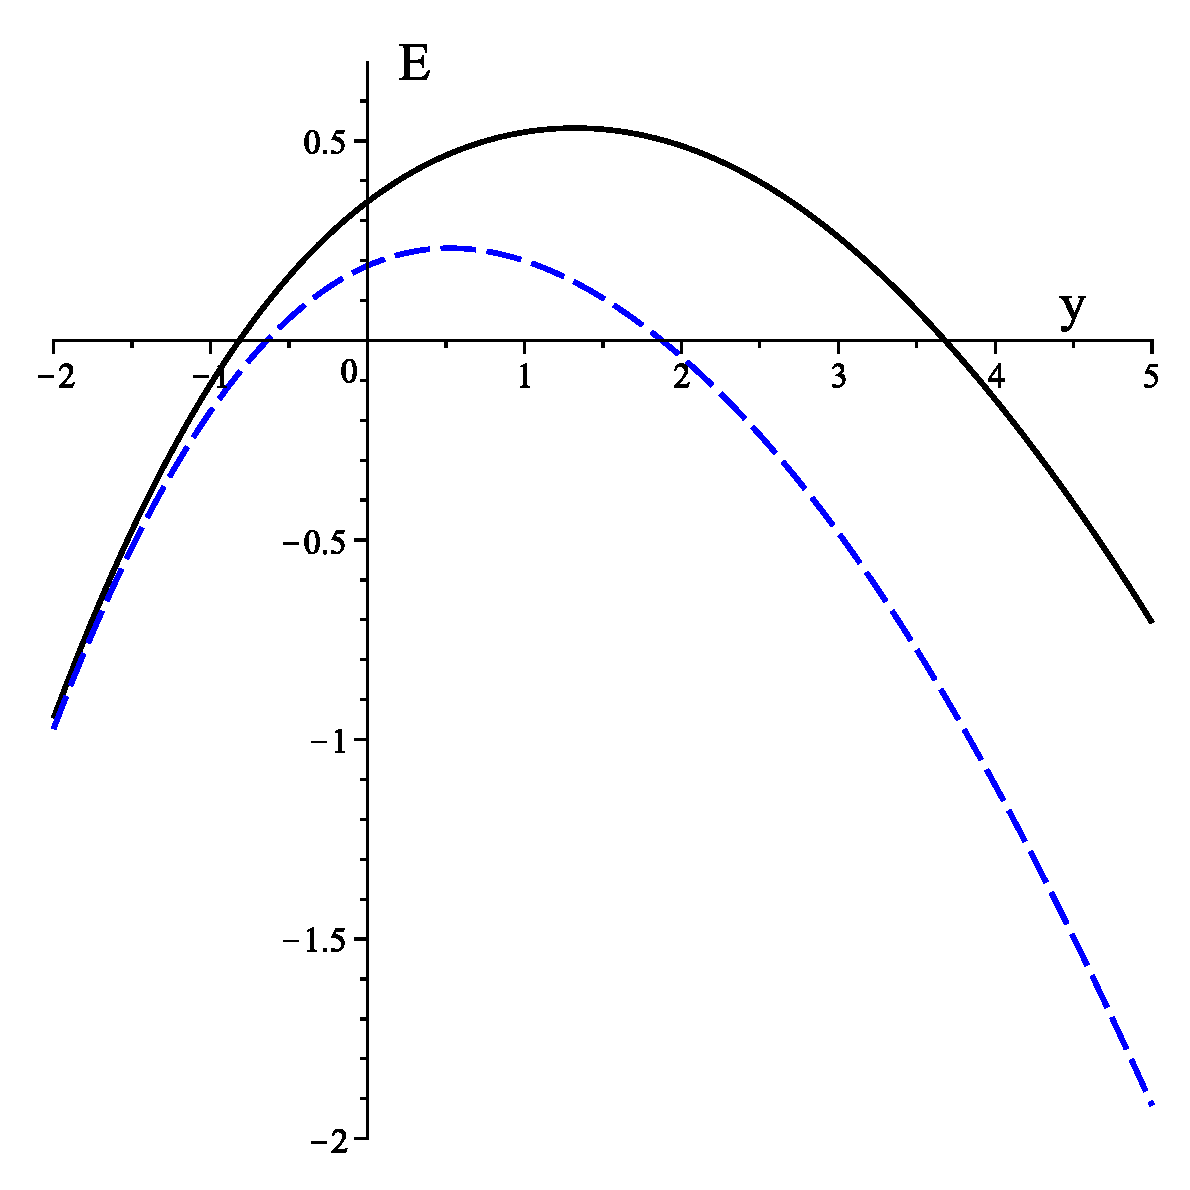
\includegraphics[width=0.5\textwidth,angle=0]{E0_vs_y}
		\centering
		\captionsetup{width=0.6\textwidth}
		\caption{Quantity $E(y,p,\mu)$ as a function of $y$ at $p=2.0$ and $\beta\mu=-2.0$ for two different values of $v^*$: Solid line (black): $v^* = 10$, Dash line (blue): $v^* = 5$.}
		\label{fig:E0_vs_y}
	\end{figure}
	
	\textit{Remark}. The estimate in~\eqref{ineq:E0} implies the following: (a) the integral in~\eqref{eq:XiInty} converges for all $p>0$ and $\mu \in \mathbb{R}$, as $a>1$; (b) for fixed $p$ and $\mu$, since $E(y,p,\mu)$ is bounded above, it has global maxima, each of which is also a local maximum.
	
	
	\section{The equation of state}
	By the known thermodynamic formula (cf.~\cite[(2.16)]{KKD20})
	\begin{equation}
		\label{def:eos}
		%P V = k_{\rm B} T \ln \Xi(\beta, \mu)
		P V = \beta^{-1} \ln \Xi(\beta, \mu)
	\end{equation}

	where $P$ is the pressure. To calculate the large $N_v$ limit in~\eqref{eq:XiInty} we first determine the global maxima of $E(y,p,\mu)$ as a function of $y \in \mathbb{R}$, and then apply the Laplace's method~\cite{Fedoryuk89}.
	
	Let $\bar{y}$ denote the point of global maximum of $E$. Then it should obey the following equation
	\begin{equation}
		\label{def:E1}
		E_1(y,p,\mu) := \frac{\partial}{\partial y} E(y,p,\mu) = 0.
	\end{equation}
	By~\eqref{def:E} and~\eqref{def:K}, the explicit expression for $E_1$ is
	\begin{equation}
		E_1(y,p,\mu) = -\frac{y}{p} + \frac{K_1(y,p,\mu)}{K(y,p,\mu)},
	\end{equation}	
	and the equation for the extremum of $E(y,p,\mu)$ can be rewritten in the form~(cf.~\cite[(2.19)]{KKD20})
	\begin{equation}
		\label{eq:bar_y}
		-\frac{y}{p} + \frac{K_1(y,p,\mu)}{K(y,p,\mu)} = 0,
	\end{equation}
	where
	\begin{equation}
		K_1(y,p,\mu) := \frac{\partial}{\partial y} K(y,p,\mu) = \sum_{n=0}^{\infty} \frac{n (v^*)^n}{n!} \exp[(y+\beta\mu)n - \frac{ap}{2}n^2].
	\end{equation}
	As $K$, $K_1$, and $p$ all take on strictly positive values, the solution $\bar{y}$ to equation~\eqref{eq:bar_y} is also strictly positive.
	Typical behavior of $E_1(y,p,\mu)$ as a function of $y$ in the single-phase domain is illustrated in Fig.~\ref{fig:E1_vs_y}.
	\begin{figure}[htbp]
		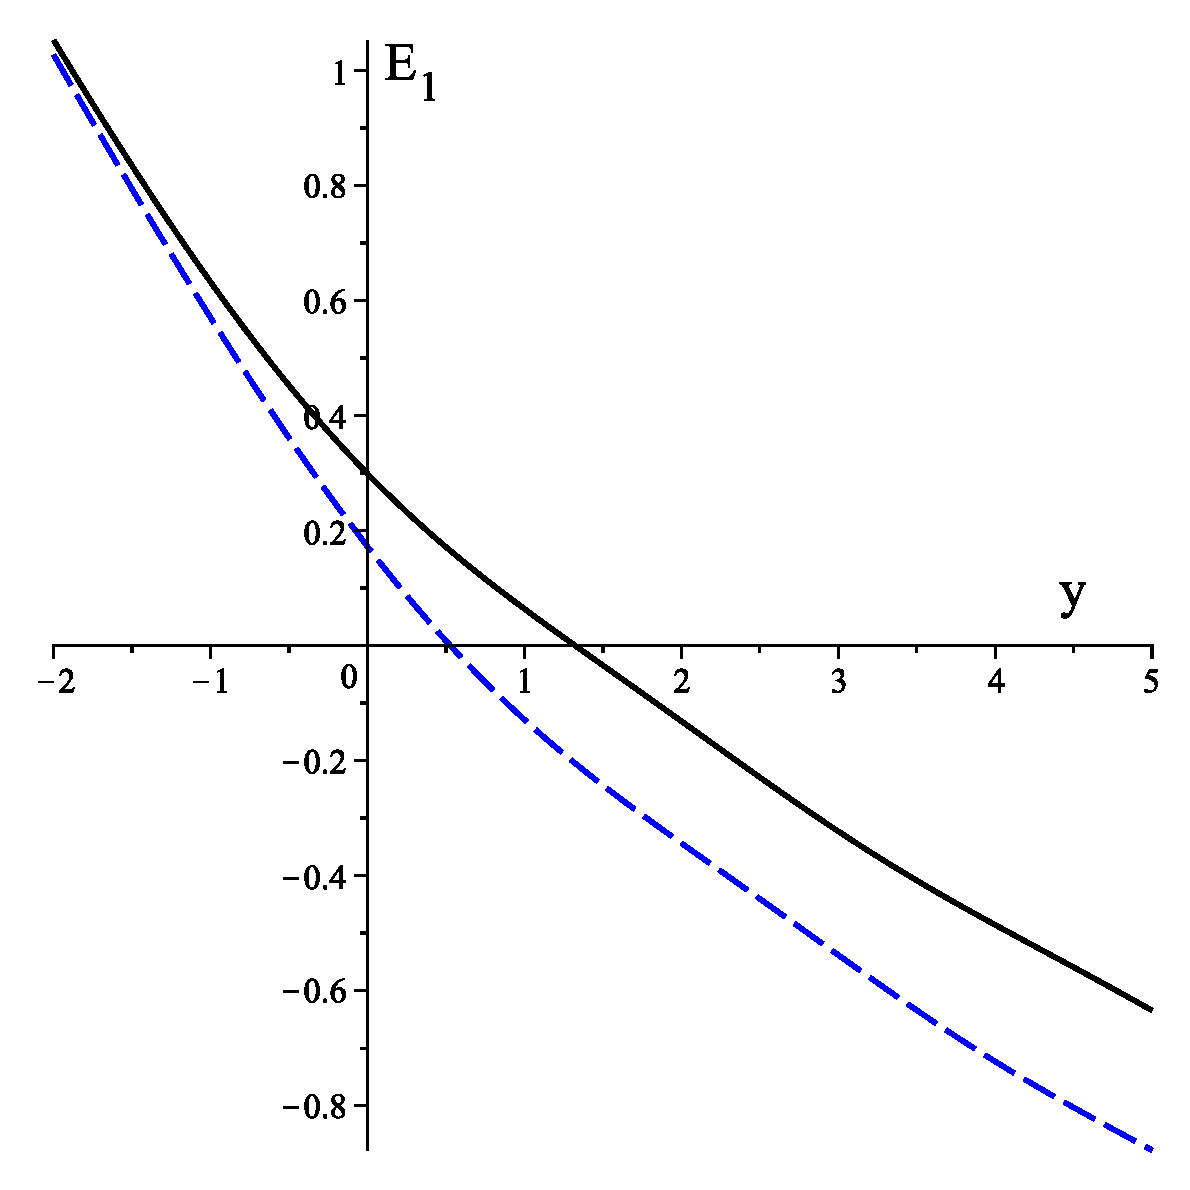
\includegraphics[width=0.5\textwidth,angle=0]{E1_vs_y}
		\centering
		\captionsetup{width=0.6\textwidth}
		\caption{Quantity $E_1(y,p,\mu)$ as a function of $y$ at $p=2.0$ and $\beta\mu=-2.0$ for two different values of $v^*$: Solid line (black): $v^* = 10$, Dash line (blue): $v^* = 5$.}
		\label{fig:E1_vs_y}
	\end{figure}
	\begin{figure}[htbp]
		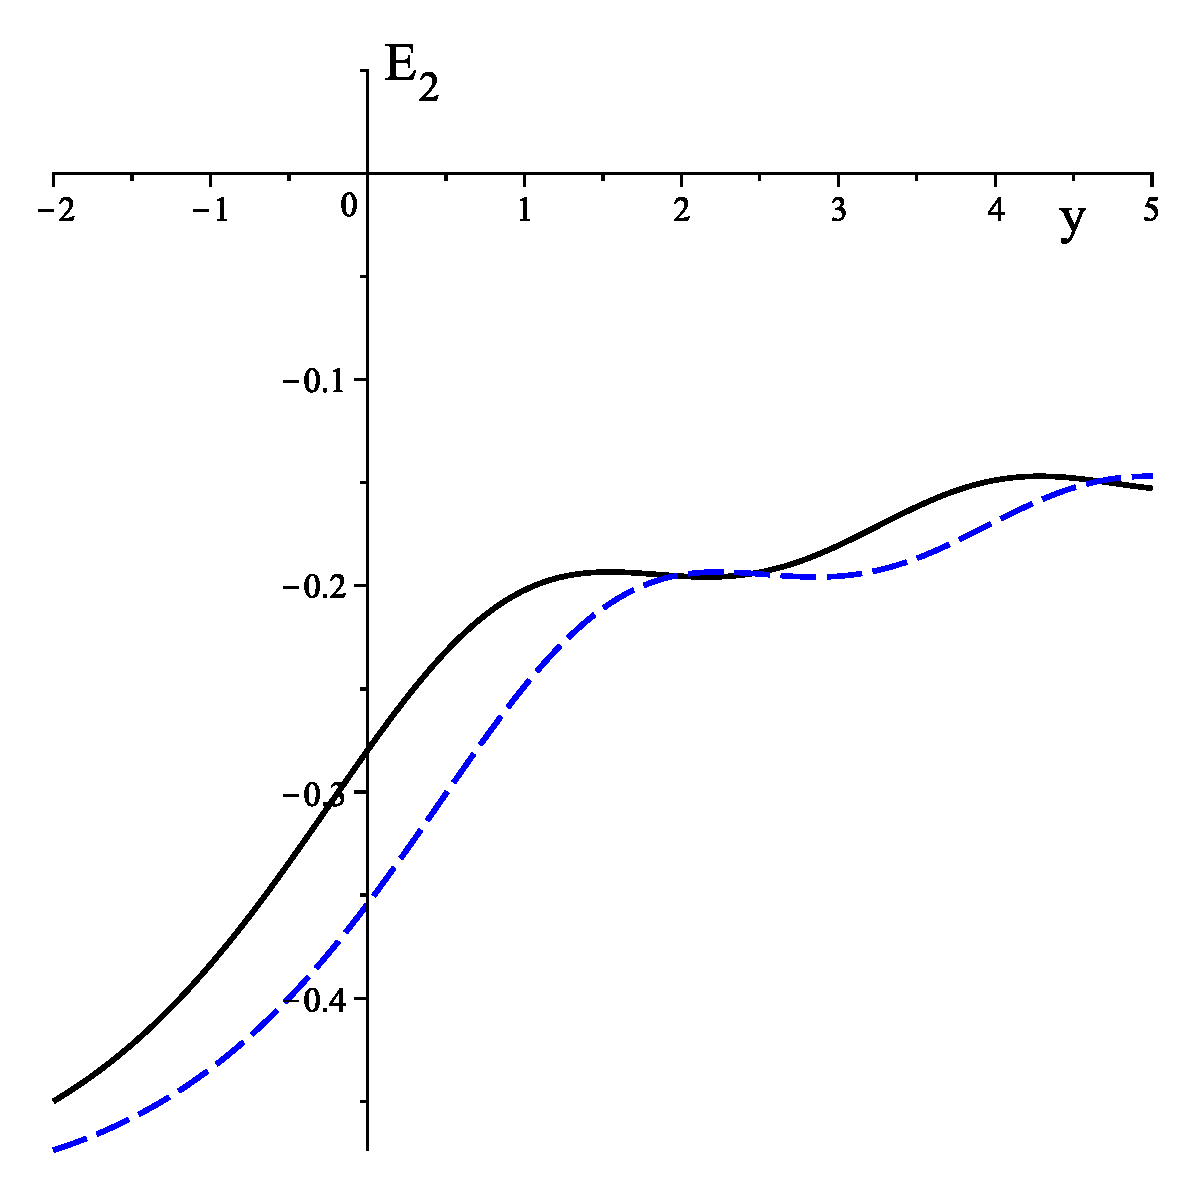
\includegraphics[width=0.5\textwidth,angle=0]{E2_vs_y}
		\centering
		\captionsetup{width=0.6\textwidth}
		\caption{Quantity $E_2(y,p,\mu)$ as a function of $y$ at $p=2.0$ and $\beta\mu=-2.0$ for two different values of $v^*$: Solid line (black): $v^* = 10$, Dash line (blue): $v^* = 5$.}
		\label{fig:E2_vs_y}
	\end{figure}
	
	\textbf{Definition}. We say that $(p, \mu)$ belongs to a single-phase domain if $E(y,p,\mu)$ has a unique global maximum $\bar{y} \in \mathbb{R}$ such that
	\begin{equation}
		E_2(\bar{y}, p, \mu) := \frac{\partial^2}{\partial y^2} E(y,p,\mu)\big|_{y=\bar{y}} < 0.
	\end{equation}
	An explicit expression for $E_2(y,p,\mu)$ reads (cf.~\cite[(20)]{KD22})
	\begin{equation}
		E_2(y,p,\mu) = -\frac{1}{p} + \frac{K_2(y,p,\mu) K(y,p,\mu) - [K_1(y,p,\mu)]^2}{[K(y,p,\mu)]^2},
	\end{equation}
	where
	\begin{equation}
		K_2(y,p,\mu) := \frac{\partial}{\partial y} K_1(y,p,\mu) = \sum_{n=0}^{\infty} \frac{n^2 (v^*)^n}{n!} \exp[(y+\beta\mu)n - \frac{ap}{2}n^2].
	\end{equation}
	Typical behavior of $E_2(y,p,\mu)$ as a function of $y$ in the single-phase domain is illustrated in Fig.~\ref{fig:E2_vs_y}.
	
	\textbf{Laplace's method.} We apply the Laplace's method~\cite[(1.21)]{Fedoryuk89} to~\eqref{eq:XiInty} and arrive at~(cf.~\cite[(19)]{KD22})
	\begin{equation}
		\Xi(p,\mu) = [-p E_2(\bar{y},p,\mu)]^{-1/2} \exp[N_v E(\bar{y},p,\mu)].
	\end{equation}
	Substituting this into~\eqref{def:eos}, one gets
	\begin{equation}
		P V = k_{\rm B}T \left[-\frac{1}{2} \ln(-p E_2(\bar{y},p,\mu)) + N_v E(\bar{y},p,\mu)\right].
	\end{equation}
	The first term in the square brackets in the right-hand side of the last equation can be neglected in the limit of large $N_v$, and we arrive at (cf.~\cite[(2.27)]{KKD20})
	\begin{equation}
		P v \beta = E(\bar{y},p,\mu),
	\end{equation}
	or
	\begin{equation}
		P^* = T^* E(\bar{y},T^*,\mu^*).
	\end{equation}
	We have obtained the equation of state expressing the pressure $P$ as a function of temperature $T$ (through variable $p$) and chemical potential $\mu$, $P = P(T, \mu)$. We accounted that the quantity $\bar{y}$, which is selected from the condition to maximize $E$ at given $T$ and $\mu$, is a function of $T$ and $\mu$, $\bar{y} = \bar{y}(p,\mu)$. The problem here is that we cannot get the solution to~\eqref{eq:bar_y} in an analytic form. Still we can get some results numerically and obtain graphics.
	
	
	\section{Entropy}
	By thermodynamic formulas for the grand canonical ensemble
	\begin{equation}
		S = -\left(\frac{\partial \Omega}{\partial T}\right)_{V,\mu} = V\left(\frac{\partial P}{\partial T}\right)_{\mu}
	\end{equation}
	where $\Omega = -k_{\rm B}T \ln \Xi$ is the grand potential. The reduced entropy reads
	\begin{equation}
		S^* := \frac{S}{N_v k_{\rm B}} = \frac{v}{k_{\rm B}} \left(\frac{\partial P}{\partial T}\right)_{\mu}
	\end{equation}
	


\section{The special function $K_0$ and its integral representation}

\be\label{KOZ}
K_0(z)=\sum_{n\ge0}\frac1{n!}\,\e^{zn-an^2}
\ee
Note that sum in \eqref{KOZ} is precisely of the same functional form as that in the definition \eqref{ZGR} of the grand partition function up to replacements
\be
N\to n,\qquad z\to\e^{-z},\MM{and}Z_n\to\e^{-an^2}.
\ee

The integral representation of $K_0(z)$ is given by
\be
K_0(z)=\frac1{2\sqrt\pi}\int_{-\infty}^\infty\e^{-\frac{x^2}4}
\mbox{exp}\left(\e^{z+ix\sqrt a}\right),
\ee
or, in the form of a manifestly real integral,
\be\label{KOR}
K_0(z)=\frac1{2\sqrt\pi}\int_{-\infty}^\infty\e^{-\frac{x^2}4}
\mbox{exp}\left[\e^z\cos(x\sqrt a\,)\right]
\cos\left[\e^z\sin(x\sqrt a\,)\right].
\ee

Can you calculate the asymptotic behavior as $z\to+\infty$ of two last integrals?

I have succeeded to calculate the leading $z\to+\infty$ asymptotics only for two integrals
\be
K_0^{(a)}(z) = \frac1{2\sqrt\pi} \int_{-\infty}^\infty\e^{-\frac{x^2}4}
\mbox{exp}\left[\e^z\cos(x\sqrt a\,)\right]\qquad\mbox{and}\qquad
\ee
\be
K_0^{(b)}(z) = \frac1{2\sqrt\pi} \int_{-\infty}^\infty\e^{-\frac{x^2}4}
\cos\left[\e^z\sin(x\sqrt a\,)\right]
\ee
resulting from \eqref{KOR} by deleting one of the last two factors.

The leading asymptotics are the following
\begin{equation}
	K_0^{(a)}(z) \sim \frac{\exp({\rm e}^z)}{\sqrt{2 {\rm e}^z}}, \quad \text{as } z \to +\infty
\end{equation}
and
\begin{equation}
	K_0^{(b)}(z) \sim \sqrt{\frac{2}{\pi {\rm e}^z}} \cos({\rm e}^z - \pi/4), \quad \text{as } z \to +\infty.
\end{equation}
	
	\appendix
	
	\section{\label{sec:app1} Explicit derivation of $E(y,p,\mu)$ and $K(y,p,\mu)$}
	In this appendix, the explicit transformations through Eqs.~(2.11)--(2.15) is presented. Substituting the Gaussian integral~\eqref{eq:gaussInt} into~\eqref{eq:XiPi}, one proceeds as follows
	\begin{eqnarray}
		\Xi 
		&=& 
		\sum_{\varrho \in \mathbb{N}_0^{N_v}} \sqrt{\frac{N_v}{2\pi p}} \int\limits_{-\infty}^{\infty} \exp(-N_v \frac{y^2}{2p}) 
		\prod\limits_{l=1}^{N_v} \frac{(v^*)^{\varrho_l}}{\varrho_l !} 
		\exp[(y + \beta\mu) \varrho_l - \frac{ap}{2}\varrho_l^2] {\rm d}y
		\nonumber\\
		&=&
		\sqrt{\frac{N_v}{2\pi p}} \sum_{\varrho_1=0}^{\infty} \ldots \sum_{\varrho_{N_v}=0}^{\infty} 
		\int\limits_{-\infty}^{\infty} {\rm e}^{-N_v \frac{y^2}{2p}} 
		\prod\limits_{l=1}^{N_v} \frac{(v^*)^{\varrho_l}}{\varrho_l !} 
		\exp[(y + \beta\mu) \varrho_l - \frac{ap}{2}\varrho_l^2] {\rm d}y
		\nonumber\\
		&=&
		\sqrt{\frac{N_v}{2\pi p}} \int\limits_{-\infty}^{\infty} {\rm e}^{-N_v \frac{y^2}{2p}}
		\left\{ 
			\sum_{\varrho_1=0}^{\infty} \frac{(v^*)^{\varrho_1}}{\varrho_1 !} \exp[(y + \beta\mu) \varrho_1 - \frac{ap}{2}\varrho_1^2] 
		\right\}
		\nonumber\\
		&& 
		\times \ldots \times 
		\left\{ 
			\sum_{\varrho_{N_v}=0}^{\infty} \frac{(v^*)^{\varrho_{N_v}}}{\varrho_{N_v} !} \exp[(y + \beta\mu) \varrho_{N_v} - \frac{ap}{2}\varrho_{N_v}^2] 
		\right\}
		{\rm d}y
		\nonumber\\
		&=&
		\sqrt{\frac{N_v}{2\pi p}} \int\limits_{-\infty}^{\infty} {\rm e}^{-N_v \frac{y^2}{2p}}
		\exp( \ln \left\{\sum_{n=0}^{\infty} \frac{(v^*)^{n}}{n!} \exp[(y + \beta\mu)n - \frac{ap}{2}n^2] \right\}^{N_v} ) {\rm d}y
		\nonumber\\
		&=&
		\sqrt{\frac{N_v}{2\pi p}} \int\limits_{-\infty}^{\infty}
		\exp 
		\left\{ N_v 
			\left[ -\frac{y^2}{2p} + 
			\ln(\sum_{n=0}^{\infty} \frac{(v^*)^{n}}{n!} {\rm e}^{(y + \beta\mu)n - \frac{ap}{2}n^2}) 
			\right] 
		\right\} {\rm d}y,
	\end{eqnarray}
	and arrives at Eqs.~\eqref{eq:XiInty}, \eqref{def:E}, and~\eqref{def:K}
	\begin{equation}
		\Xi = \sqrt{\frac{N_v}{2\pi p}} \int\limits_{-\infty}^{\infty}
		\exp 
		\left\{ N_v 
		\left[ -\frac{y^2}{2p} + 
		\ln K(y,p,\mu) 
		\right] 
		\right\}.
	\end{equation}

	
	%\bibliographystyle{elsarticle-num}
	%\bibliography{books,articles}
	
	\bibliographystyle{JHEPm}
	\bibliography{Mbank}
		
\end{document} 
